\section{Direct and Indirect Effects}
\label{sec:direct}

Two or 3 paragraphs describing how genetic wage effects can be direct or indirect.

Describe what the sources of direct or indirect, and why a composition of education-focused genes would matter for this.

Define the causal effects, and then the estimation equation.

Say that it is not identified

\subsection{Minimum School Leaving Age (MSLA)}

Describe that education (or at least one year) is randomly assigned for compliers of the increased minimum school leavers' age law, which in 1972 raised the minimum age one can leave school (legally) from 15 to 16.
Following this, GCSE completion rate immediately increased by 6 percentage points, and average education years by 0.2 for those born around the cusp of the September 1957.

\begin{figure}[h!]
    \centering
    \singlespacing
    \caption{Mean Education Completion Around the MSLA Rise.}
    \begin{subfigure}[b]{0.495\textwidth}
        \centering
        %\caption{GCSE Completion Rate.}
        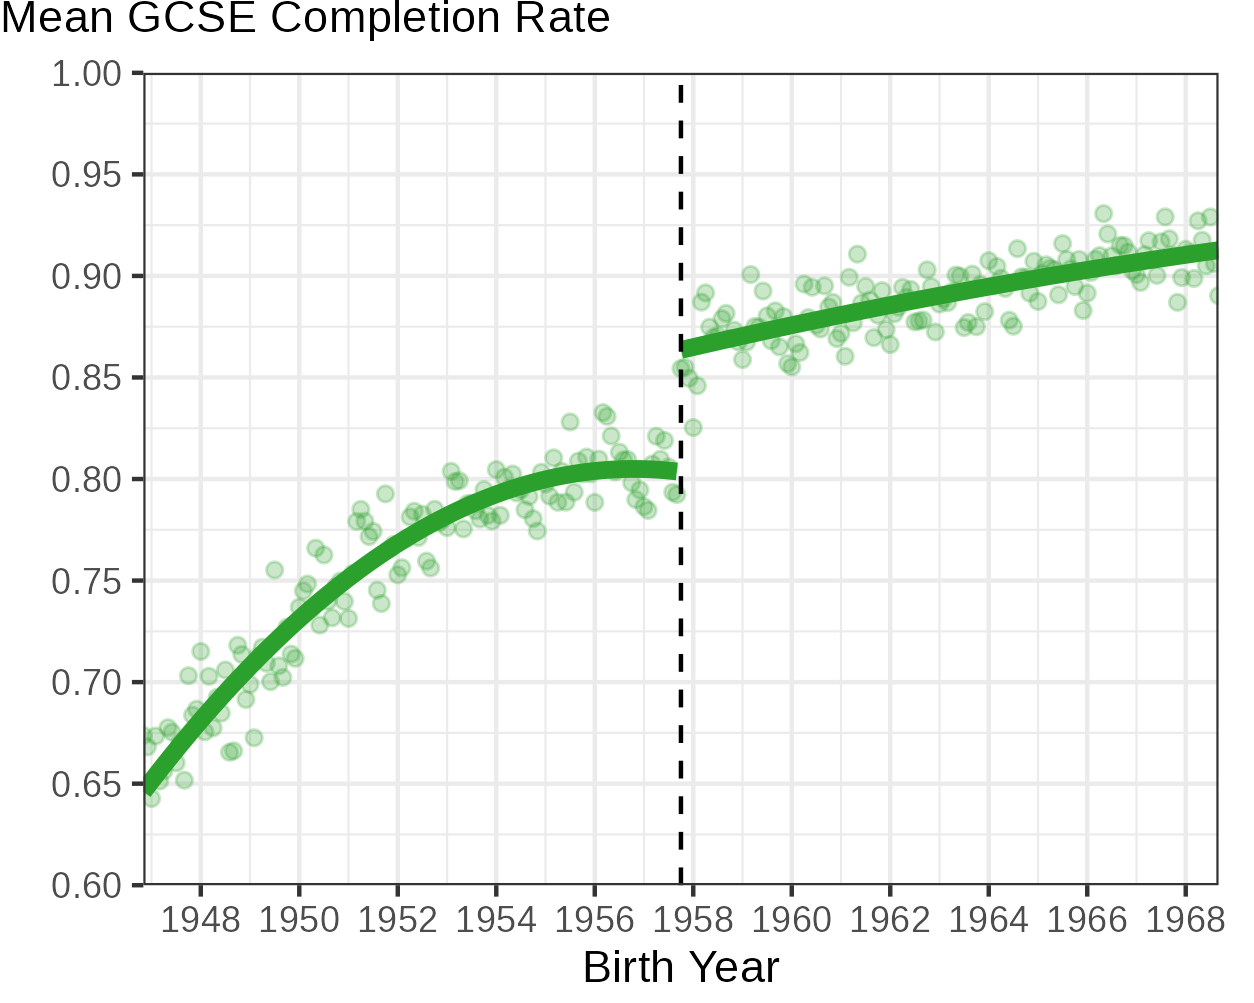
\includegraphics[width=\textwidth]{sections/figures/rosla-gcse.png}
    \end{subfigure}
    \begin{subfigure}[b]{0.495\textwidth}
        \centering
        %\caption{Mean Education Years.}
        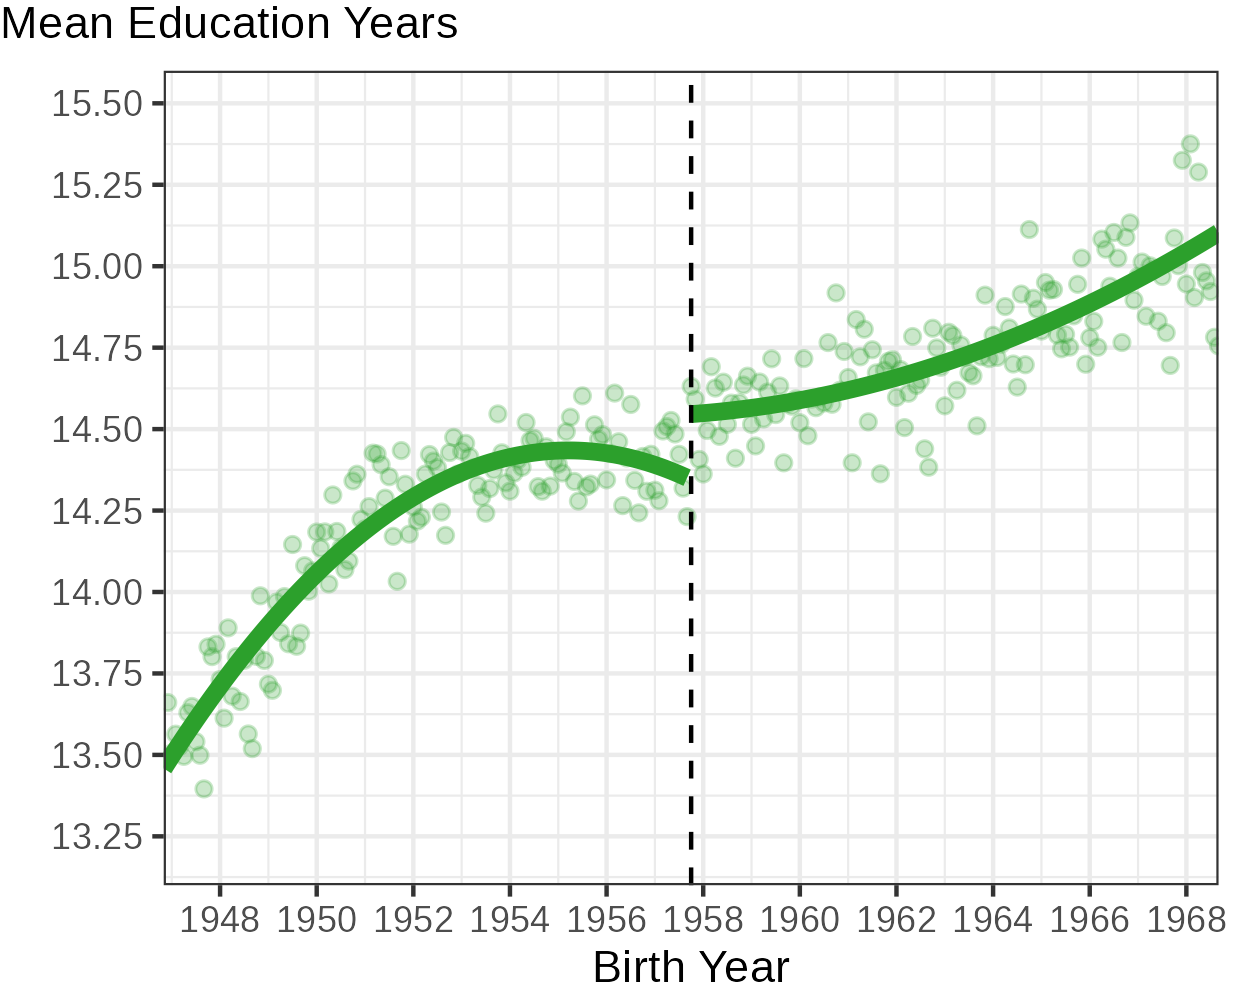
\includegraphics[width=\textwidth]{sections/figures/rosla-edyears.png}
    \end{subfigure}
    \label{fig:rosla}
    \vspace{-1cm}
    \justify
    \footnotesize
    \textbf{Note}:
    These numbers are calculated using the entire UKB sample; the sibling subsample has too few data points for inference around the law change cut-off.
\end{figure}

Further writing about how identifying 

\begin{table}[!h]
    \singlespacing
    \centering
    \caption{Effects of the MSLA Change.}
    \centerline{
    \begin{tabular}{l c c c c c c c c}
        \\[-1.8ex]\hline \hline \\[-1.8ex] 
        & \multicolumn{4}{c}{First-stage.}
            & \multicolumn{4}{c}{Reduced form.}\\
        \cmidrule(lr){2-5} \cmidrule(lr){6-9}
        Outcome: & \multicolumn{2}{c}{GCSE}       & \multicolumn{2}{c}{Education} & \multicolumn{2}{c}{Hourly} & \multicolumn{2}{c}{Annual}  \\
        & \multicolumn{2}{c}{Completion} & \multicolumn{2}{c}{Years}     & \multicolumn{2}{c}{Wage}   & \multicolumn{2}{c}{Income} \\
        \cmidrule(lr){2-5} \cmidrule(lr){6-9}
        & (1) & (2) & (3) & (4) & (5) & (6) & (7) & (8) \\
        \\[-1.8ex]\hline \\[-1.8ex]
        % latex table generated in R 4.5.2 by xtable 1.8-4 package
% Wed Feb 18 13:33:14 2026
 MSLA Effect & 0.198 & 0.208 & 0.260 & 0.316 & 0.004 & 0.010 & 0.001 & 0.014 \\ 
    & (0.006) & (0.004) & (0.029) & (0.029) & (0.003) & (0.003) & (0.008) & (0.003) \\ 
  $F$-statistics & 1108 & 2761 & 82 & 121 & 2 & 10 & 0 & 25 \\ 
  
        \\[-1.8ex]\hline \\[-1.8ex]
    \end{tabular}
    }
    \vspace{-0.25cm}
    \label{tab:msla-firststage}
    \justify
    \footnotesize
    \textbf{Note:}
    Talk about it.
    Note this is among the entire sample, and not the sibling analysis subsample.
\end{table}

\subsection{Returns to Education}

\begin{table}[!h]
    \singlespacing
    \centering
    \caption{Returns to Education, Motivated by MSLA Change.}
    \centerline{
    \begin{tabular}{l c c c c c c c c}
        \\[-1.8ex]\hline \hline \\[-1.8ex] 
        & \multicolumn{4}{c}{OLS.}
            & \multicolumn{4}{c}{MLSA IV.}\\
        \cmidrule(lr){2-5} \cmidrule(lr){6-9}
        & (1) & (2) & (3) & (4) & (5) & (6) & (7) & (8) \\
        \\[-1.8ex]\hline \\[-1.8ex]
        \multicolumn{9}{l}{\textbf{Outcome:} Log Occupation Hourly Wage} \\
        % latex table generated in R 4.5.2 by xtable 1.8-4 package
% Wed Feb 18 13:33:16 2026
 Education years $\geq 16$ & 0.192 & 0.193 &   &   & 0.061 & 0.073 &   &   \\ 
    & (0.009) & (0.008) &   &   & (0.008) & (0.016) &   &   \\ 
  Education years &   &   & 0.034 & 0.034 &   &   & 0.047 & 0.048 \\ 
    &   &   & (0.002) & (0.002) &   &   & (0.004) & (0.010) \\ 
  
        \\[-1.8ex]\hline \\[-1.8ex]
        \multicolumn{9}{l}{\textbf{Outcome:} Log Occupation Annual Income} \\
        % latex table generated in R 4.5.2 by xtable 1.8-4 package
% Wed Feb 18 13:33:19 2026
 Education years $\geq 16$ & 0.196 & 0.188 &   &   & 0.040 & 0.070 &   &   \\ 
    & (0.012) & (0.009) &   &   & (0.004) & (0.014) &   &   \\ 
  Education years &   &   & 0.033 & 0.032 &   &   & 0.031 & 0.046 \\ 
    &   &   & (0.002) & (0.002) &   &   & (0.002) & (0.010) \\ 
  \\[-1.8ex]\hline \\[-1.8ex] Linear trends & Yes &   & Yes &   & Yes &   & Yes &   \\ 
  Polynomial trends &   & Yes &   & Yes &   & Yes &   & Yes \\ 
  Observations & 86,349 & 149,796 & 86,349 & 149,796 & 86,349 & 149,796 & 86,349 & 149,796 \\ 
  
        \\[-1.8ex]\hline \\[-1.8ex]
    \end{tabular}
    }
    \vspace{-0.25cm}
    \label{tab:msla-secondstage}
    \justify
    \footnotesize
    \textbf{Note:}
    Talk about it.
    Note this is among the entire sample, and not the sibling analysis subsample.
\end{table}

\begin{table}[!h]
    \singlespacing
    \centering
    \caption{Returns to Higher Education.}
    \centerline{
    \begin{tabular}{l c c c c c c c c}
        \\[-1.8ex]\hline \hline \\[-1.8ex] 
        & \multicolumn{4}{c}{OLS.}
            & \multicolumn{4}{c}{MLSA IV.}\\
        \cmidrule(lr){2-5} \cmidrule(lr){6-9}
        & (1) & (2) & (3) & (4) & (5) & (6) & (7) & (8) \\
        \\[-1.8ex]\hline \\[-1.8ex]
        \multicolumn{9}{l}{\textbf{Outcome:} Log Occupation Hourly Wage} \\
        % latex table generated in R 4.5.2 by xtable 1.8-4 package
% Wed Feb 18 13:33:16 2026
 Education years $\geq 16$ & 0.192 & 0.193 &   &   & 0.061 & 0.073 &   &   \\ 
    & (0.009) & (0.008) &   &   & (0.008) & (0.016) &   &   \\ 
  Education years &   &   & 0.034 & 0.034 &   &   & 0.047 & 0.048 \\ 
    &   &   & (0.002) & (0.002) &   &   & (0.004) & (0.010) \\ 
  
        \\[-1.8ex]\hline \\[-1.8ex]
        \multicolumn{9}{l}{\textbf{Outcome:} Log Occupation Annual Income} \\
        % latex table generated in R 4.5.2 by xtable 1.8-4 package
% Wed Feb 18 13:33:19 2026
 Education years $\geq 16$ & 0.196 & 0.188 &   &   & 0.040 & 0.070 &   &   \\ 
    & (0.012) & (0.009) &   &   & (0.004) & (0.014) &   &   \\ 
  Education years &   &   & 0.033 & 0.032 &   &   & 0.031 & 0.046 \\ 
    &   &   & (0.002) & (0.002) &   &   & (0.002) & (0.010) \\ 
  \\[-1.8ex]\hline \\[-1.8ex] Linear trends & Yes &   & Yes &   & Yes &   & Yes &   \\ 
  Polynomial trends &   & Yes &   & Yes &   & Yes &   & Yes \\ 
  Observations & 86,349 & 149,796 & 86,349 & 149,796 & 86,349 & 149,796 & 86,349 & 149,796 \\ 
  
        \\[-1.8ex]\hline \\[-1.8ex]
    \end{tabular}
    }
    \vspace{-0.25cm}
    \label{tab:msla-secondstage}
    \justify
    \footnotesize
    \textbf{Note:}
    Talk about it.
    Note this is among the entire sample, and not the sibling analysis subsample.
\end{table}




Show some tables here for the MSLA first-stage, and how they get that education returns are roughly the same as correlational estimates.


Lead into to estimating mediation equations in specifications which include the MSLA instrument, where possible, and correlation returns to education when noted.
Indeed, education is not randomly assigned so that causal estimates of mediation effects will be affected by not identifying causal returns to education (see \citealt{hogan2025causal})





\subsection{Old Writing:}

Given the inherent limitations of identifying causal effects of education—particularly the absence of a credible external instrument in my setting—I adopt a sensitivity-analysis-based approach to interpret the role of education and genetic predictors in shaping later-life outcomes. Rather than asserting point identification, I rely on a range of plausible estimates for the return to education, derived from both conventional cross-sectional regressions and family fixed effects models (e.g., sibling comparison).

The benchmark correlational estimate suggests that each additional year of education is associated with approximately a 6-7\% increase in income. However, when controlling for family fixed effects, the estimated return falls to around 4\%, consistent with prior literature showing downward bias in FE models due to measurement error, but still providing a plausible lower bound.

I then use these benchmarks to evaluate the direct effect of the polygenic index (PGI) for education on income. Conditioning on educational attainment, the direct effect of the education PGI becomes statistically indistinguishable from zero. Given that the total effect of the PGI on income remains positive, this implies that the indirect effect of the PGI—operating through education—is dominant. Indeed, under the assumption that the true causal return to education is at least as large as the family fixed effects estimate, the implied indirect effect is even stronger, reinforcing the conclusion that the direct (non-educational) effect of the PGI on later-life income is negligible.

In this way, the sensitivity analysis does not rely on strong causal identification of the education-income link, but instead uses conservative bounds to demonstrate the robustness of a mediation pattern in which the genetic influence of the education PGI operates almost entirely through educational attainment.

Explain this with a simple Roy model.

Note that this now allows for a choice channel, when previously it had not.
